%%%%%%%%%%%%%%%%%%%%%%%%%%%%%%%%%%%%%%%%%%%%%%%%%%%%%%%%%%%%%%%%%%%%%%%%

%%% LaTeX Template for AAMAS-2024 (based on sample-sigconf.tex)
%%% Prepared by the AAMAS-2024 Program Chairs based on the version from AAMAS-2023. 

%%%%%%%%%%%%%%%%%%%%%%%%%%%%%%%%%%%%%%%%%%%%%%%%%%%%%%%%%%%%%%%%%%%%%%%%

%%% Start your document with the \documentclass command.


%%% == IMPORTANT ==
%%% Use the first variant below for the final paper (including auithor information).
%%% Use the second variant below to anonymize your submission (no authoir information shown).
%%% For further information on anonymity and double-blind reviewing, 
%%% please consult the call for paper information
%%% https://www.aamas2024-conference.auckland.ac.nz/calls/submission-instruction/

\documentclass[sigconf]{aamas} 
%\documentclass[sigconf,anonymous]{aamas} 


%%% Load required packages here (note that many are included already).

\usepackage{balance} % for balancing columns on the final page

\usepackage{csquotes}
\usepackage{pbox}

%%%%%%%%%%%%%%%%%%%%%%%%%%%%%%%%%%%%%%%%%%%%%%%%%%%%%%%%%%%%%%%%%%%%%%%%

%%% AAMAS-2024 copyright block (do not change!)

\setcopyright{ifaamas}
\acmConference[AAMAS '24]{Proc.\@ of the 23rd International Conference
on Autonomous Agents and Multiagent Systems (AAMAS 2024)}{May 6 -- 10, 2024}
{Auckland, New Zealand}{N.~Alechina, V.~Dignum, M.~Dastani, J.S.~Sichman (eds.)}
\copyrightyear{2024}
\acmYear{2024}
\acmDOI{}
\acmPrice{}
\acmISBN{}

%%%%%%%%%%%%%%%%%%%%%%%%%%%%%%%%%%%%%%%%%%%%%%%%%%%%%%%%%%%%%%%%%%%%%%%%

%%% == IMPORTANT ==
%%% Use this command to specify your EasyChair submission number.
%%% In anonymous mode, it will be printed on the first page.

\acmSubmissionID{<<EasyChair submission id>>}

%%% Use this command to specify the title of your paper.

\title[AAMAS-2024 CybMASDE]{CybMASDE: A Development Environment For Cyberdefense Multi-Agent Systems}

%%% Provide names, affiliations, and email addresses for all authors.

\author{Julien Soulé}
\affiliation{
  \institution{Univ. Grenoble Alpes}
  \city{Valence}
  \country{France}}
\email{julien.soule@lcis.grenoble-inp.fr}

\author{Jean-Paul Jamont}
\affiliation{
  \institution{Univ. Grenoble Alpes}
  \city{Valence}
  \country{France}}
\email{jean-paul.jamont@lcis.grenoble-inp.fr}

\author{Michel Occello}
\affiliation{
  \institution{Univ. Grenoble Alpes}
  \city{Valence}
  \country{France}}
\email{michel.occello@lcis.grenoble-inp.fr}

\author{Louis-Marie Traonouez}
\affiliation{
  \institution{Thales Land and Air Systems, BU IAS}
  \city{Rennes}
  \country{France}}
\email{louis-marie.traonouez@thalesgroup.com}

\author{Paul Théron}
\affiliation{
  \institution{AICA IWG}
  \city{La Guillermie}
  \country{France}}
\email{paul.theron@orange.fr}

%%% Use this environment to specify a short abstract for your paper.

% ----------------------------------
%   Notes
% ----------------------------------

% Novel applications and interactive systems are particularly welcome.

% Demonstrations of interest include:
%   - Systems implementing agents in real-world applications in areas such as transportation, robotics, grid, e-commerce, health care, military, etc.
%   - Systems using agents in virtual settings, which include simulation systems, VR, and games.
%   - Systems supporting the development of agents, which include development environments and tools to assist developers in the specification, design, implementation, and testing of agent systems.


% Each Demo submission must consist of a short paper, a video, and, for student projects, a supervisor endorsement note. The submission requirements are the following.

% 1. Paper. The paper should include a maximum of four pages and be structured as follows:
% - Pages 1-2 should describe the system to be demonstrated. More precisely, the authors are encouraged to discuss the application domain, the problem scenario, the technology used, the agent/multi-agent techniques involved, the system’s innovations, the system’s live and interactive aspects, etc.
% - Page 3 should include bibliographic references.
% - Page 4 should provide the organisers with a list of requirements for the demo setting at the conference.

% 2. Video. The paper should contain a URL linking to a demonstration video of no more than 5 minutes in duration (QuickTime or YouTube format). The video should include the following elements:
% - Introduction: Introduce the concept/system.
% - Aim: What is the target group for the system?
% - Main features: Present the system’s main features and discuss the benefits as well as innovations.
% - Development: Architecture overview, agent-based techniques, and technologies used for development.
% - Demo. Execution of the system that highlights its features and benefits.

% The evaluation criteria are:
% - Relevance to the AAMAS conference
% - Significance and originality
% - Live demo presentation and technical quality
% - Video content and presentation
% - Maturity and readiness for demonstration
% - Potential for public interaction
% - Potential impact in the intended application domain

% ----------------------------------


\begin{abstract}
We propose the \emph{Cyberdefense Multi-Agent Systems Development Environment} (CybMASDE), a tool for helping in the design, implementation and assessing of cyber-defender agents that tackle cyber-attacker agents in a networked system. It is based on the CybORG simulation and emulation network environment, that enables powering the design phase with agents' training. It aims to bring practical control and assist means from scenario modeling until the deployment of a specified Cyberdefense Multi-Agent System.
First, we introduce CybMASDE and its motivations regarding the gaps it intends to fill. Then, we give an technical overview of the CybMASDE functioning. Finally, we discuss about case studies with successful application of CybMASDE.
\end{abstract}

%%% The code below was generated by the tool at http://dl.acm.org/ccs.cfm.
%%% Please replace this example with code appropriate for your own paper.


%%% Use this command to specify a few keywords describing your work.
%%% Keywords should be separated by commas.

\keywords{Cyberdefense, Multi-Agent systems, Design tool, Network application-level, Simulation, Emulation, Demo}

%%%%%%%%%%%%%%%%%%%%%%%%%%%%%%%%%%%%%%%%%%%%%%%%%%%%%%%%%%%%%%%%%%%%%%%%

%%% Include any author-defined commands here.
         
\newcommand{\BibTeX}{\rm B\kern-.05em{\sc i\kern-.025em b}\kern-.08em\TeX}

%%%%%%%%%%%%%%%%%%%%%%%%%%%%%%%%%%%%%%%%%%%%%%%%%%%%%%%%%%%%%%%%%%%%%%%%

\begin{document}

%%% The following commands remove the headers in your paper. For final 
%%% papers, these will be inserted during the pagination process.

\pagestyle{fancy}
\fancyhead{}

%%% The next command prints the information defined in the preamble.

\maketitle 

%%%%%%%%%%%%%%%%%%%%%%%%%%%%%%%%%%%%%%%%%%%%%%%%%%%%%%%%%%%%%%%%%%%%%%%%

% Describe the system to be demonstrated. More precisely, the authors are encouraged to discuss the application domain, the problem scenario, the technology used, the agent/multi-agent techniques involved, the system’s innovations, the system’s live and interactive aspects, etc.

\section{Introduction}


% Context
%   - application domain
In some heterogenous and distributed systems such as drone swarms, smart cities or company infrastructures, centralized Cyberdefense systems may show limitations to address the increasing complexity of cyber-threats regarding constraints of fast environmental changes, embedded systems, limited human action, unstable communication and so on. Works carried out for \emph{Autonomous Intelligent Cyberdefense Agents} (AICA)~\cite{Kott2023}, have fostered a multi-agent approach of Cyberdefense where cyber-defender collaborating agents are deployed on a networked system making up a Cyberdefense Multi-Agent System (CMAS).
We envision that type of Multi-Agent System (MAS) in a scenario as a blue team that aims to achieve Cyberdefense goals to fight against a red team of cyber-attacker agents and tackle them and their impact on the networked environment and regular users represented as a green team.
That vision falls into the \emph{Autonomous Cyber Operation} (ACO) research works such as in the \emph{Cyber Operation Research Gym}~\cite{Standen2021} (CybORG), an environment for developing and researching in autonomous cyber-agents.

% Problem
%   - problem scenario

Yet, from a developer point-of-view no methodological means have been pushed forward to guide and assist the development a CMAS that ensures intended Cyberdefense in the considered networked system described in a scenario.

% Hypothesis / Contribution:
%   - technology used
%   - the system's innovations

Based upon CybORG, we introduce CybMASDE, an interactive tool to help the development process of a CMAS regarding the environmental constraints and Cyberdefense goals. The underlying development approach relies on simulation for designing and filtering relevant CMAS models in a scenario; and emulation for implementing and assessing those models in the real networked system described in the scenario.
In simulation, means have been set up to take advantage of a bottom-up approach by using Multi-Agent Reinforcement Learning (MARL) to bring out emergent successful CMAS models or fine-tuning parametrized ones. Those can be analyzed to understand their resulting organization specifications with the help of a behavioral analysis view in a GUI.

% Results

Even though CybMASDE is at an early development stage, feedbacks received from non expert users in academic and industrial contexts, express its quick utilization for convincing results with few skills required compared to CybORG.


%%%%%%%%%%%%%%%%%%%%%%%%%%%%%%%%%%%%%%%%%%%%%%%%%%%%%%%%%%%%%%%%%%%%%%%%

\section{Positioning and contribution}

Since a CMAS is a new concept, CybMASDE was originally thought after having analyzed that available application-level network simulation or emulation environments do not fully take into account the MAS paradigm to benefit from collective AI techniques such as self/re-organization or MARL; and the methodological needs regarding the users' interactions. A summary of the conducted analysis is presented in Table \ref{tab:litterature_review_summary}.

% CLSE, CybORG, CyberBattleSim, NeSSi2, NaSim, CYST, YANG

\begin{table}[t]
	\caption{Overview of desired properties coverage in the main considered environments}
	\label{tab:litterature_review_summary}
	\begin{tabular}{lccccccccc}\toprule
		% \pbox{20cm}{Environment \\ designed for}
    {} & \textit{\cite{Standen2021}} & \textit{\cite{Standen2021}} & \textit{\cite{Standen2021}} & \textit{\cite{Standen2021}} & \textit{\cite{Standen2021}} & \textit{\cite{Standen2021}} & \textit{\cite{Standen2021}} & \textit{\cite{Standen2021}} & \textit{\cite{Standen2021}} \\
    
    \midrule

    {Simulation} & \checkmark &  &  &  &  &  &  &  &  \\
    {Emulation} &  & \checkmark &  &  &  &  &  &  &  \\
    {Blue team} &  &  &  &  &  &  &  &  &  \\
    {Red team} &  &  &  & \checkmark &  &  &  &  &  \\
    {Green team} &  &  &  &  &  & \checkmark &  &  &  \\
    {MARL} &  &  &  &  &  &  &  &  &  \\
    {GUI} &  &  & \checkmark &  &  &  &  &  & \checkmark \\
    {Generic} &  &  & \checkmark &  &  &  &  &  & \checkmark \\
    {Extendable} &  &  & \checkmark &  &  &  &  &  & \checkmark \\
    \pbox{20cm}{Organization \\ analysis} &  &  & \checkmark &  &  &  &  &  & \checkmark \\

    \bottomrule

	\end{tabular}
\end{table}

CybMASDE is mainly motivated by the limited genericity, the lack of acquaintance with our vision of a scenario, the virtual absence of organization analysis tools, and the weak presence of user interactions means.
CybMASDE is intended to bring forward the necessary means for researcher to apply a methodological approach based on an iterative lifecycle alternating between simulation for pre-designing CMAS models and emulation for validating them.
In that regard, we chose to extend CybORG capabilities to meet our requirements since it is the closest to them, in particular for its high fidelity to application-level network simulation.

In simulation is the integration of an API to integrate our approach helps to properly model the problem in the scenario by defining the network nodes (router, servers, embedded systems), the green team (as an indicator of the network health) and the red team (such as malware programs, worms inspired from framework such as the MITRE ATT\&CK TTPs). Consequently, the flexibility in simulation, leaves room for designing a CMAS models through various resolution approaches ranging from a fully top-down design to bottom-up mechanisms including MARL techniques. Those are analyzed regarding their emergent organization and quantitatively assessed and filtered according to their cumulative rewards.
The contribution in emulation is a semi-automated process to reproduce the networked system as a set of networked virtual machines or emulated nodes, and transfer agents of each team into those for validating them in real conditions.

%%%%%%%%%%%%%%%%%%%%%%%%%%%%%%%%%%%%%%%%%%%%%%%%%%%%%%%%%%%%%%%%%%%%%%%%

\section{Technical description}

CybMASDE is a web application comprising a Python backend including a modified version of CybORG integrating our development approach, and an Angular frontend interface for a more accessible user interaction.

The backend can be presented through five modules.
The \textit{scenario store} which contains pre-defined json file configurations of nodes, networks, agents, or even all-in-one complete scenarios . Configuration files are compliant to a flexible format enabling the description of various software and hardware characteristics. 
The \textit{simulation API} comprises the endpoint for using the bakcend modules. It enables updating and loading the configuration library components to compose/use a scenario configuration, creating a simulation instance of the currently loaded scenario and following its execution through analysis tools.
The \textit{simulation engine} which is the modified CybORG simulator that runs the simulation instance by instantiating all of the required objects described in the scenario file configuration. It also launches the running of agents and handle the updating of the instantiated environment depending on applied actions.
The \textit{emulation engine} that runs the emulation instance by creating and configuring all the nodes described in the configuration file as networked virtual machines using Ancible. It requires some manual configuration for provisioning the host machines. It also handle the creation, monitoring and launching the described agents of each team thanks to a success/failure signal system.
The \textit{organization specification engine} that is a side-tool for automating the design of a CMAS by generating the suited specifications that foster its performance. It relies on MARL for extracting the best suited specified organization models from trained agents behaviors. The agent training can also consists in refining parametrized behavior according to pre-defined MAS architectures such as coalition based or hierarchy ones.

The frontend has several components endowing the backend endpoints of the \textit{simulation API} within a single GUI.
The \textit{scenario store} interface allows manual updating and loading of the configuration files in text-editors. A loaded scenario is displayed in the left side panel.
The \textit{simulation engine} is played when configuring a simulation instance specifying the number of episodes and iterations for agents' mechanisms that requires training. It also retrieves and displays real-time and complementary data concerning the running of the execution in order to filtering under performant CMAS models in simulation.
The \textit{emulation engine} is played when configuring the generation of an emulation instance. It asks for confirmation of using the generated emulation and deployment plan from backend. That YAML file indicates the operations to be executed for creating the networked environment how agents should be deployed. Then, the data retrieved after launching are also displayed for ultimately filtering successful CMAS models.
The \textit{organization specification engine} is played as an option during the simulation configuration of a scenario to enable the generation of the organization specifications at the end of simulation. It should be preferably chosen when the blue agents' behavior models requires some training, and an overall picture of agents interaction as organization is not obvious. These specifications can be exported as a json file for later implementation of MAS models.

\begin{figure}[h]
  \centering
  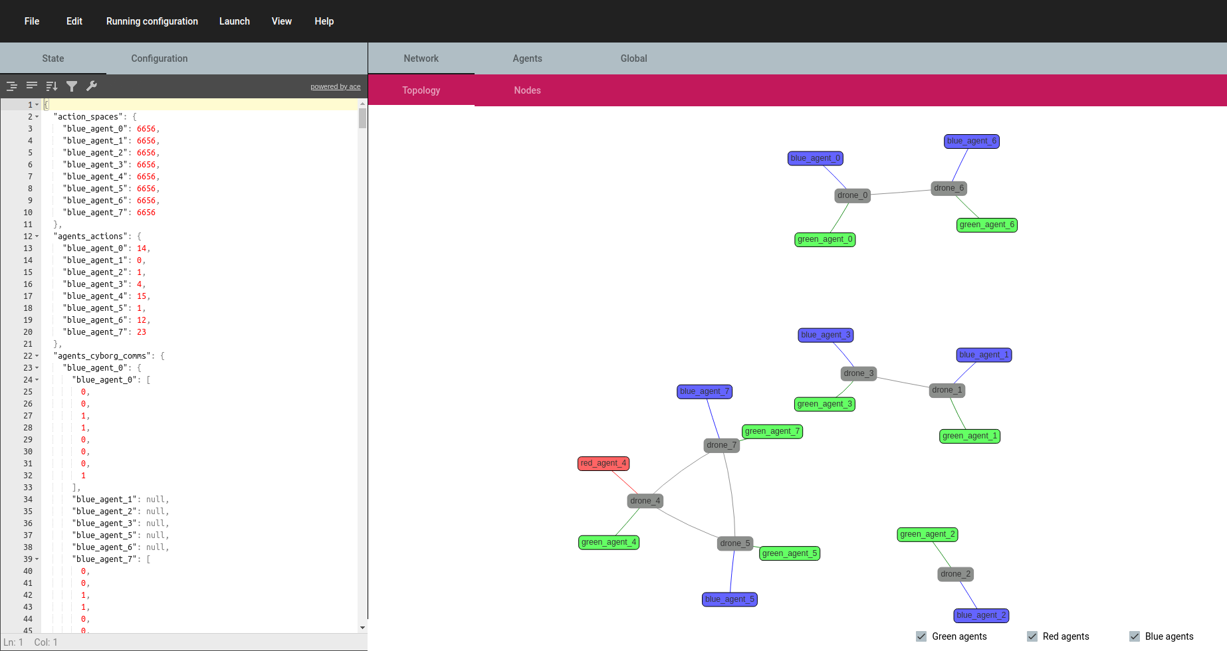
\includegraphics[width=\linewidth]{CybMASDE_main_view.png}
  \caption{Main view in CybMASDE}
  \label{fig:screenshot}
  \Description{Screenshot of the main view in NeSSi2: The GUI enables the creation and administration of arbitrary networks and node configurations. After the setup process is finished, an agent-based simulation back-end (“CommunicationPlatform”) executes the simulation and the results are stored in a database.}
\end{figure}

%%%%%%%%%%%%%%%%%%%%%%%%%%%%%%%%%%%%%%%%%%%%%%%%%%%%%%%%%%%%%%%%%%%%%%%%

\section{Successful utilization}

CybMASDE has been initiated and used through a student research project as an experimental platform to study the organizational issues of a CMAS regarding given deployment and operational constraints when aiming to reach intended Cyberdefense goals. In that regard, we addressed the third CAGE Challenge\cite{cage_challenge_3_announcement2022} that consist in creating a suited CMAS to protect an ad hoc drone swarm network being cyber-attacked by malware programs for it meets inherent embedded and distributed properties.

Furthermore, the successful utilization of CybMASDE by non-expert students for fictitious company infrastructures scenarios in projects, have expressed CybMASDE to be a relevant support for fast development of tailored CMAS matching the researchers needs with limited required skills by focusing on relevant users' interactions.

Aside of the academic contribution, CybMASDE is also used within an industrial context in a micro-architecture Kubernetes scenario for addressing specific cyber-attacks in pod orchestration. CybMASDE is also to be used for the development of AICA-like CMAS allowing to adapt the theoretical architectural polyvalent vision of an AICA to the deployment and operational constraints of various IoBT related environments.

CybMASDE is envisioned as an Open Source participative research project to be freely used in research and development contexts.


%%%%%%%%%%%%%%%%%%%%%%%%%%%%%%%%%%%%%%%%%%%%%%%%%%%%%%%%%%%%%%%%%%%%%%%%

\section{Conclusion}

CybMASDE was proposed to provide methodological help for designing, implementing and assessing collaborating cyber-defender agents to reach given Cyberdefense goals in distributed embedded systems. Its backend is based upon the CybORG simulation framework and engine ensuring a good fidelity level to reality while taking advantage of MARL to generate or refine CMAS models.
The CybMASDE's GUI assists users in the iterative process of the design, implementation, assessing, and analyze phases. Finally, as an early research project, CybMASDE is in use both in academic and industrial contexts.

%%%%%%%%%%%%%%%%%%%%%%%%%%%%%%%%%%%%%%%%%%%%%%%%%%%%%%%%%%%%%%%%%%%%%%%% 

% TODO: ?
% \begin{acks}
% \end{acks}

%%%%%%%%%%%%%%%%%%%%%%%%%%%%%%%%%%%%%%%%%%%%%%%%%%%%%%%%%%%%%%%%%%%%%%%%

\newpage

\bibliographystyle{ACM-Reference-Format} 
\bibliography{local_references}

%%%%%%%%%%%%%%%%%%%%%%%%%%%%%%%%%%%%%%%%%%%%%%%%%%%%%%%%%%%%%%%%%%%%%%%%

\newpage
\phantom{ }
\newpage

\section*{Requirements for the demo setting}




%%%%%%%%%%%%%%%%%%%%%%%%%%%%%%%%%%%%%%%%%%%%%%%%%%%%%%%%%%%%%%%%%%%%%%%%

\end{document}

%%%%%%%%%%%%%%%%%%%%%%%%%%%%%%%%%%%%%%%%%%%%%%%%%%%%%%%%%%%%%%%%%%%%%%%%

